\chapter{Results}
\label{results}
\graphicspath{{Results/Images/}}

\section{Regolith launched from the longest edge of the asteroid}
\label{regolith_longest_edge}
The results that we'll discuss in this section pertain to the case of regolith launched from the longest edge of the asteroid, modeled as an ellipsoid.

\subsection{Dynamics without Solar perturbations}
\label{regolith_longest_edge_without_solar}
...to be added later...

\subsection{Dynamics with Solar perturbations}
\label{regolith_longest_edge_with_solar}
In this case, the simulation accounted for perturbations from the irregular gravity field of the asteroid, the \gls{SRP}, and the \gls{STBE}. Within this category, there are 4 distinct sets of simulations, each for a particle with different Area-to-Mass ratio. These are mentioned in \Cref{tab:area_to_mass_ratio}. The material with a density of 3.2 [g/cm$^3$] is low-density Olivine and the one with 7.5 [g/cm$^3$] is Iron-Nickel alloy \cite{passiveSorting}. The mineral Olivine can be found on asteroids and has been discovered on asteroid Itokawa through transmission electron microscope analysis of samples returned by the Hayabusa spacecraft \cite{olivineHayabusa}. Iron-Nickel alloy is found to be most abundant in metallic meteorites \cite{ironAlloy}.
%%%
\begin{table}[]
\centering
\captionsetup{justification=centering}
\caption{Particle Area-to-Mass ratios}
\label{tab:area_to_mass_ratio}
\begin{tabular}{|l|c|c|c|}
\hline
Code    & \multicolumn{1}{l|}{Particle radius {[}cm{]}} & \multicolumn{1}{l|}{Density {[}g/cm$^3${]}} & \multicolumn{1}{l|}{Area-to-Mass ratio {[}m$^2$/kg{]}} \\ \hline
LoGSP-1     &   1.0     &   3.2     &   0.0234      \\ \hline
LoGSP-2     &   1.0     &   7.5     &   0.01        \\ \hline
LoGSP-3     &   5.0     &   3.2     &   0.0047      \\ \hline
LoGSP-4     &   5.0     &   7.5     &   0.002       \\ \hline
\end{tabular}
\end{table}
%%%

For each of the four types of particles mentioned in \Cref{tab:area_to_mass_ratio}, the initial conditions for lofting the regolith are varied in the same manner. These initial conditions are mentioned as follows. The asteroid revolves around the Sun in an equatorial circular orbit at a distance of 1.0 \gls{AU}. Four different initial Solar phase angles were considered for the simulation – 45.0, 135.0, 225.0 315.0 [deg], to account for the four different quadrants where the Sun could be with respect to the asteroid. For each case in \Cref{tab:area_to_mass_ratio}, a total of 72 particles were launched from the surface of the asteroid, each in a different direction (defined using the launch declination and azimuth angles). The launch declination angle, measured from the zenith, was kept constant at 45.0 [deg] for all the particles. The launch azimuth, measured \gls{CCW} from the direction pointing to north, was varied at a resolution of 5.0 [deg] starting from 0.0 [deg] all the way up to 355.0 [deg]. Each particle was launched, in their specified direction, with different velocities ranging from 1.0 [m/s] to 16.0 [m/s] (measured with respect to the asteroid-centric rotating frame) at a resolution of 1.0 [m/s]. So basically, every combination of an initial Solar phase angle, initial launch azimuth, and initial launch velocity corresponds to a unique trajectory for a single particle of a given Area-to-Mass ratio; Thus amounting to a total of 4608 unique trajectories. The simulations were subjected to run for a maximum of 270.0 [days] and were terminated earlier if a particular trajectory resulted in escape or surface re-impact.

\subsubsection{Case LoGSP-1}
\label{LoGSP-1}
The density of the regolith was considered to be 3.2 [g/cm$^{3}$] with a spherical shape of radius 1.0 [cm]. \Cref{fig:LoGSP_1_final_fate_histogram} gives a distribution of particles for each of the three different final fates for the regolith i.e. capture, re-impact, and escape, for different initial launch velocities and initial Solar phase angles. Irrespective of the initial Solar phase, initial launch velocities from 1.0 to 3.0 [m/s] results in particles launched in all directions to eventually re-impact the asteroid's surface. Similarly, for initial launch velocities ranging from 14.0 to 16.0 [m/s], we see that the particles always manage to escape the gravitational attraction of the asteroid. However, there is one exception to the former statement, a single particle launched with a velocity of 14.0 [m/s] at a launch azimuth of 90.0 [deg] and at an initial Solar phase angle of 315.0 [deg], re-impacts the asteroid's surface. It is interesting to note that the launch azimuth of the particle is such that it is launched in a direction that is directly opposite to the direction of rotation of the asteroid. Launch velocities from 4.0 to 13.0 [m/s] show a mixed behavior and the final fate distribution trend does not vary drastically for different initial Solar phase angles.

The number of capture cases is far less than those for escape and re-impact. For initial Solar phase of 225.0 [deg], there are no cases of regolith being captured in orbit around the asteroid. All capture cases, arranged in order of increasing launch azimuth angle, are listed in \Cref{tab:LoGSP_1_capture}. It is interesting to note that all capture cases result from when the particle is launched in a direction which is against the direction of rotation of the asteroid, bar one exception which is case index-11 in \Cref{tab:LoGSP_1_capture}.
%%%
\begin{table}[htb]
\centering
\captionsetup{justification=centering}
\caption{Initial conditions that resulted in temporary orbital capture of regolith around the asteroid. Particle code LoGSP-1.}
\label{tab:LoGSP_1_capture}
\begin{tabular}{|l|c|c|c|}
\hline
Index & \multicolumn{1}{l|}{Launch azimuth [deg]} & \multicolumn{1}{l|}{Launch velocity [m/s]} & \multicolumn{1}{l|}{Initial Solar phase angle [deg]} \\ \hline
\rowcolor[HTML]{FE996B}
1   & 5.0 & 5.0 & 315.0     \\ \hline
\rowcolor[HTML]{67FD9A}
2   & 10.0 & 9.0 & 135.0    \\ \hline
\rowcolor[HTML]{9698ED}
3   & 15.0 & 8.0 & 45.0     \\ \hline
\rowcolor[HTML]{FFCC67}
4   & 45.0 & 12.0 & 45.0    \\ \hline
\rowcolor[HTML]{96FFFB}
5   & 45.0 & 10.0 & 315.0   \\ \hline
\rowcolor[HTML]{FFCC67}
6   & 135.0 & 12.0 & 45.0   \\ \hline
\rowcolor[HTML]{96FFFB}
7   & 135.0 & 10.0 & 315.0  \\ \hline
\rowcolor[HTML]{9698ED}
8   & 165.0 & 8.0 & 45.0    \\ \hline
\rowcolor[HTML]{67FD9A}
9   & 170.0 & 9.0 & 135.0   \\ \hline
\rowcolor[HTML]{FE996B}
10  & 175.0 & 5.0 & 315.0   \\ \hline
11  & 185.0 & 5.0 & 135.0   \\ \hline
\end{tabular}
\end{table}
%%%
The capture cases which represent symmetry in terms of the launch azimuth angle are highlighted with the same color in \Cref{tab:LoGSP_1_capture}. This symmetric behavior results from the combination of two factors. First, the Sun's motion relative to the asteroid is not in an inclined plane, and secondly, the particles are launched from the equatorial tip of the ellipsoid shaped asteroid, which is a point of symmetry on the ellipsoid. The capture cases will be discussed in detail a bit further ahead.
%%%
\begin{figure}[htb]
\centering
\captionsetup{justification=centering}
% another option for includegraphics - keepaspectratio
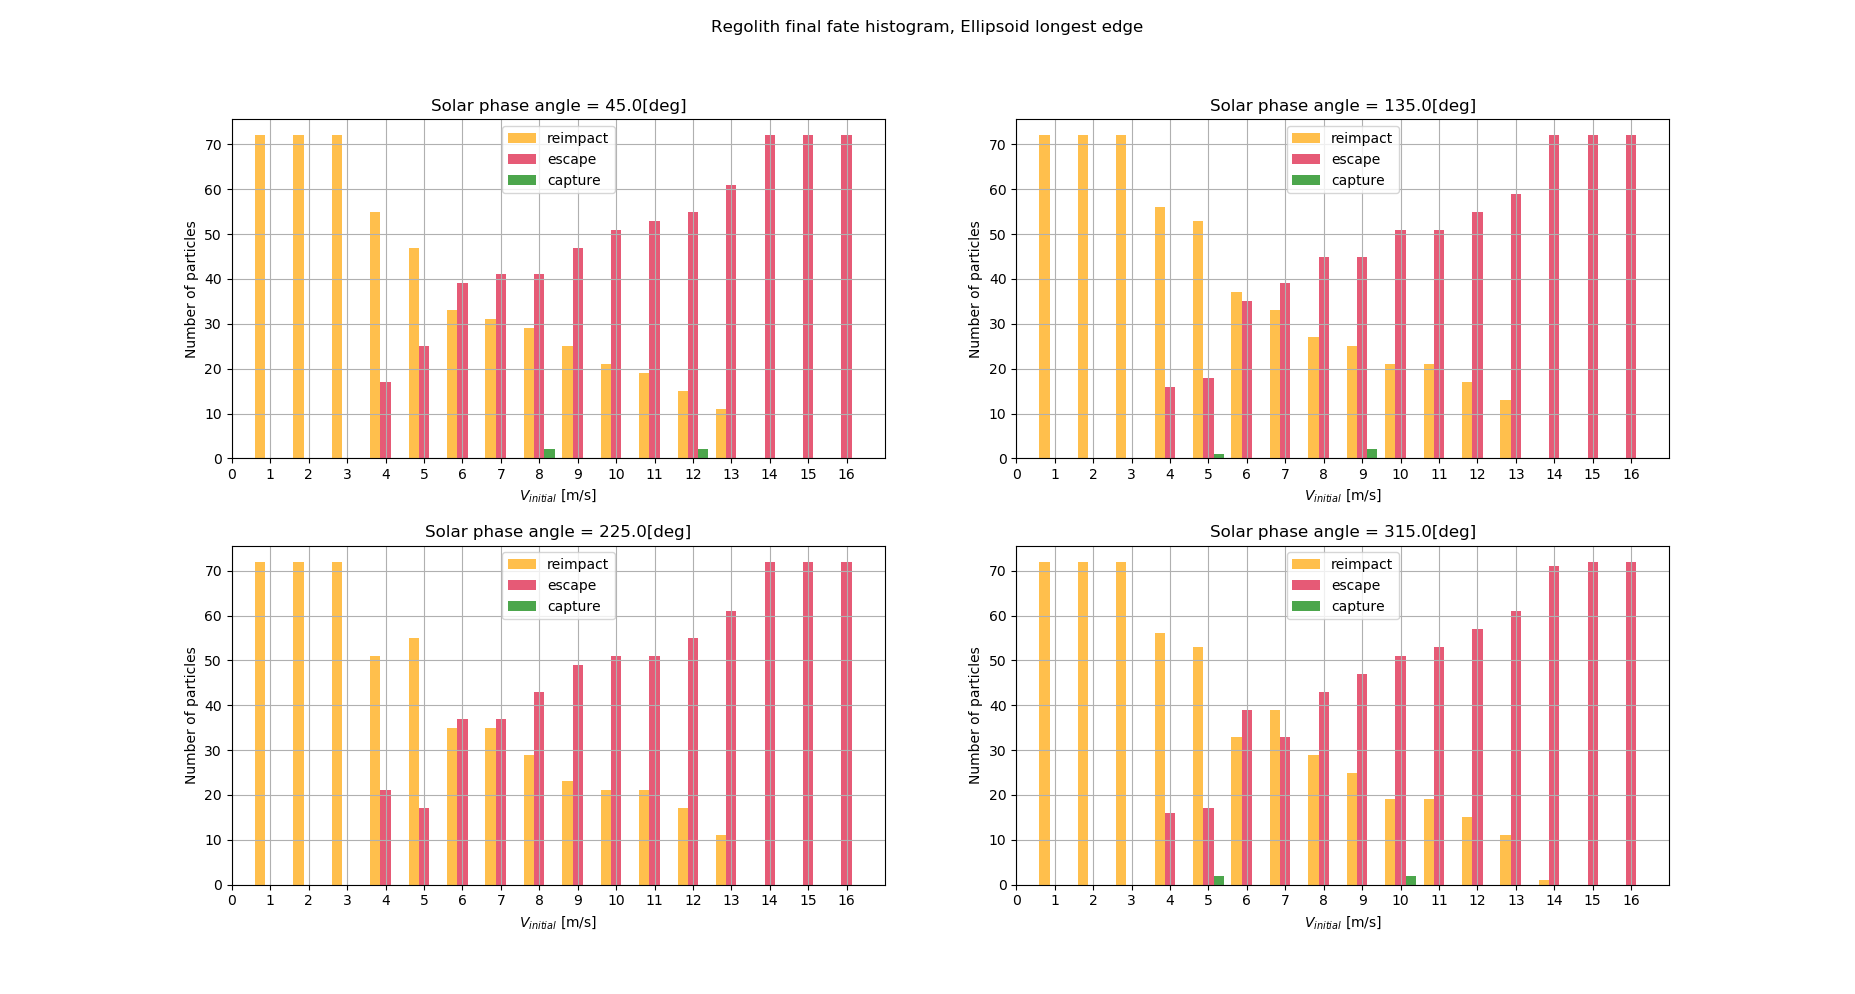
\includegraphics[angle=90, width=\textwidth, height=\textheight]{longest_edge_perturbations/3.2Density_1cmSize/final_fate_versus_launch_velocity_histogram_all_solar_phases.png}
\caption{Histogram showing the number of particles that re-impact, escape, or get captured around the asteroid, for different initial launch velocities. Particle code LoGSP-1.}
\label{fig:LoGSP_1_final_fate_histogram}
\end{figure}
\FloatBarrier
%%%
\Cref{fig:LoGSP_1_crashmap} depicts the surface distribution of regolith that re-impacts the surface when launched from the same location with different velocities and different initial Solar phase angles. The launch location is in the centre of the map, Latitude 0.0 [deg] and Longitude 0.0 [deg]. The particle distribution is the same for regions close to the launch point and for lower launch velocities up until 8.0 [m/s]. A similarity in distribution pattern is also observed around Longitude -150.0 [deg] for launch velocity of 9.0 [m/s] and around Longitude 150.0 [deg] for launch velocity of 10.0 [m/s] for the four Solar phase angles. The distribution pattern, for all launch velocities and initial Solar phases, is also symmetric about the equator. Again, the reason for this is the same as mentioned earlier for the symmetry in capture cases in \Cref{tab:LoGSP_1_capture}. Keeping the launch direction and velocity constant, we see that the distribution of regolith that re-impacts the surface does not change drastically with varying initial Solar phase angles, except for a relatively few cases. This is much easily observed in a plot of Range from the launch direction to the re-impact point versus launch azimuth for different velocities as shown in \Cref{fig:LoGSP_1_range_comparison}.

We haven't shown the range to re-impact point plots in \Cref{fig:LoGSP_1_range_comparison} for all launch velocities because the intention here is to show the qualitative behavior, which can be achieved by considering only a subset of the launch velocities that result in a re-impact scenario. The very first thing we observe is that as the launch velocity increases, the range of launch azimuth over which the regolith re-impacts the surface reduces because a higher velocity allows the regolith to enter a higher orbit (as it attains a relatively higher energy) and reduces the probability of a re-impact. Even as the velocity increases, we see that the azimuths that result in a re-impact are the ones in which the regolith is launched in a direction that is opposite to the asteroid's rotation direction. This makes sense since the regolith's energy would be reduced the most in this scenario compared to all other launch directions, thereby increasing the chances of a re-impact.

Now the primary purpose of the plots in \Cref{fig:LoGSP_1_range_comparison} (combined with \Cref{fig:LoGSP_1_crashmap}) is to depict the qualitative effect of Solar perturbations, for varying initial Solar phase angles, on the re-impact behavior of regolith compared to the case when no Solar perturbations are considered. For launch velocities of 4.0, 7.0 and 10.0 [m/s], we see that the Solar perturbations do not affect the re-impact location for cases when the particle is launched in directions opposite to that of the asteroid's rotation. However, we do see few exceptions to the former statement, most noticeably in the case of 7.0 [m/s]. But for the majority of cases where the re-impact location remains unchanged, we see from \Cref{fig:LoGSP_1_reimpact_time}, that these particles spend less than 3.0 [Hrs] in orbit which is not enough time for the Solar perturbations to act and have any significant impact on the dynamics of the particles. So in essence this is what's happening here - Particles when launched in a direction that is opposite to that of the asteroid's rotation, even at relatively high velocities such as 10.0 [m/s], loose enough energy to stay in a relatively lower orbit (see \Cref{fig:LoGSP_1_maxAltitude_reimpactscenario}) where the gravitational force of the asteroid is significantly stronger than any of the Solar perturbations and as the particle spends a very short time in orbit before re-impact, the Solar perturbations do not get enough time to affect the particle's orbit and hence the particle re-impacts the same location as it would have when no Solar perturbations were considered in the simulation. For the lower launch velocities of 4.0 and 7.0 [m/s], the differences in re-impact locations are more pronounced when the regolith is launched in the same direction as that of the asteroid's rotation. Particles gain relatively higher energy in this case, enter a higher orbit and spend enough time in there for the Solar perturbations to affect it's motion. For the case of the launch velocity of 13.0 [m/s] in \Cref{fig:LoGSP_1_range_comparison}, the velocity is high enough such that the particle does not loose enough energy when launched opposite to the asteroid's rotational direction and is able to enter a relatively higher orbit (see \Cref{fig:LoGSP_1_maxAltitude_reimpactscenario}) and stay there for a relatively longer time, as seen in \Cref{fig:LoGSP_1_reimpact_time}, which results in the Solar perturbations affecting the orbital motion and eventually the re-impact location of the regolith.
%%%
\begin{figure}[htb]
\centering
\captionsetup{justification=centering}
% another option for includegraphics - keepaspectratio
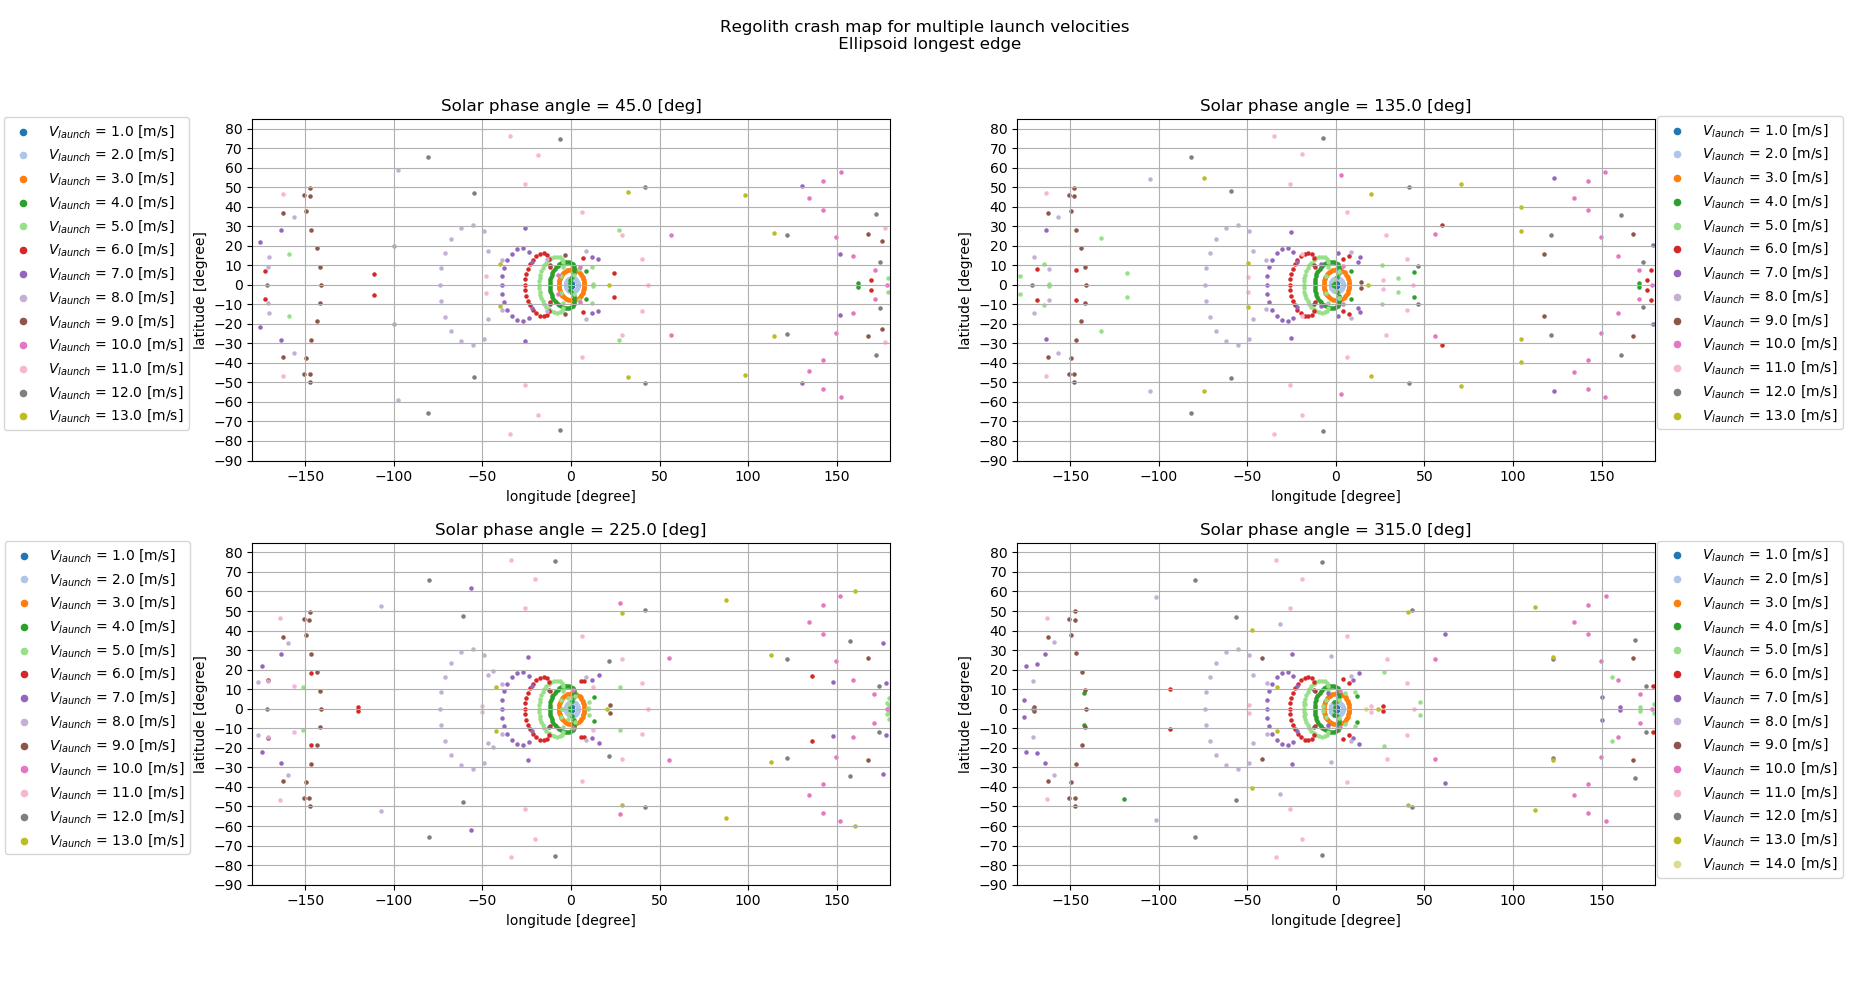
\includegraphics[angle=90, width=\textwidth, height=\textheight]{longest_edge_perturbations/3.2Density_1cmSize/crash_map_all_solar_phases.png}
\caption{Surface distribution of re-impacted regolith for different launch velocities. The launch location is \\ latitude: 0.0 [deg], longitude: 0.0 [deg]. Particle code LoGSP-1.}
\label{fig:LoGSP_1_crashmap}
\end{figure}
\FloatBarrier
%%%
%%%
\begin{figure}[htb]
\centering
\captionsetup{justification=centering}
% another option for includegraphics - keepaspectratio
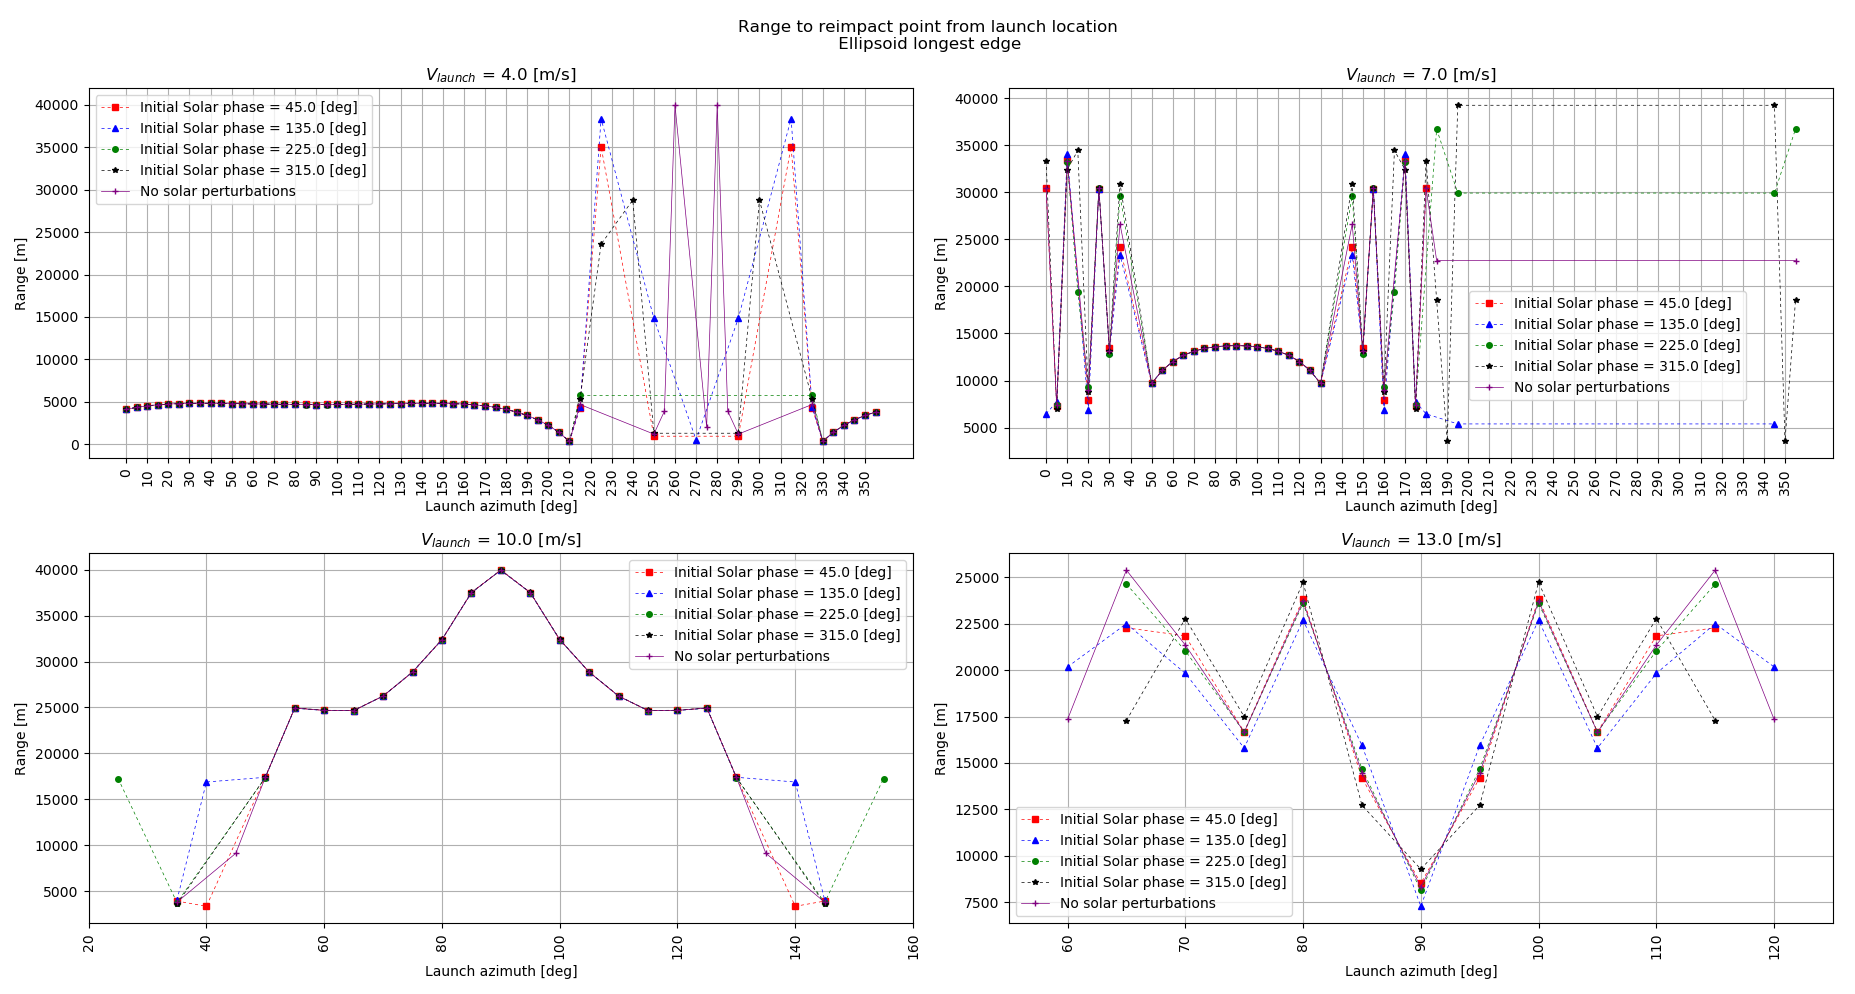
\includegraphics[angle=90, width=\textwidth, height=\textheight]{longest_edge_perturbations/3.2Density_1cmSize/reimpactRangeComparison.png}
\caption{Range to re-impact location from the launch point for different velocities. Particle code LoGSP-1.}
\label{fig:LoGSP_1_range_comparison}
\end{figure}
\FloatBarrier
%%%
%%%
\begin{figure}[htb]
\centering
\captionsetup{justification=centering}
% another option for includegraphics - keepaspectratio
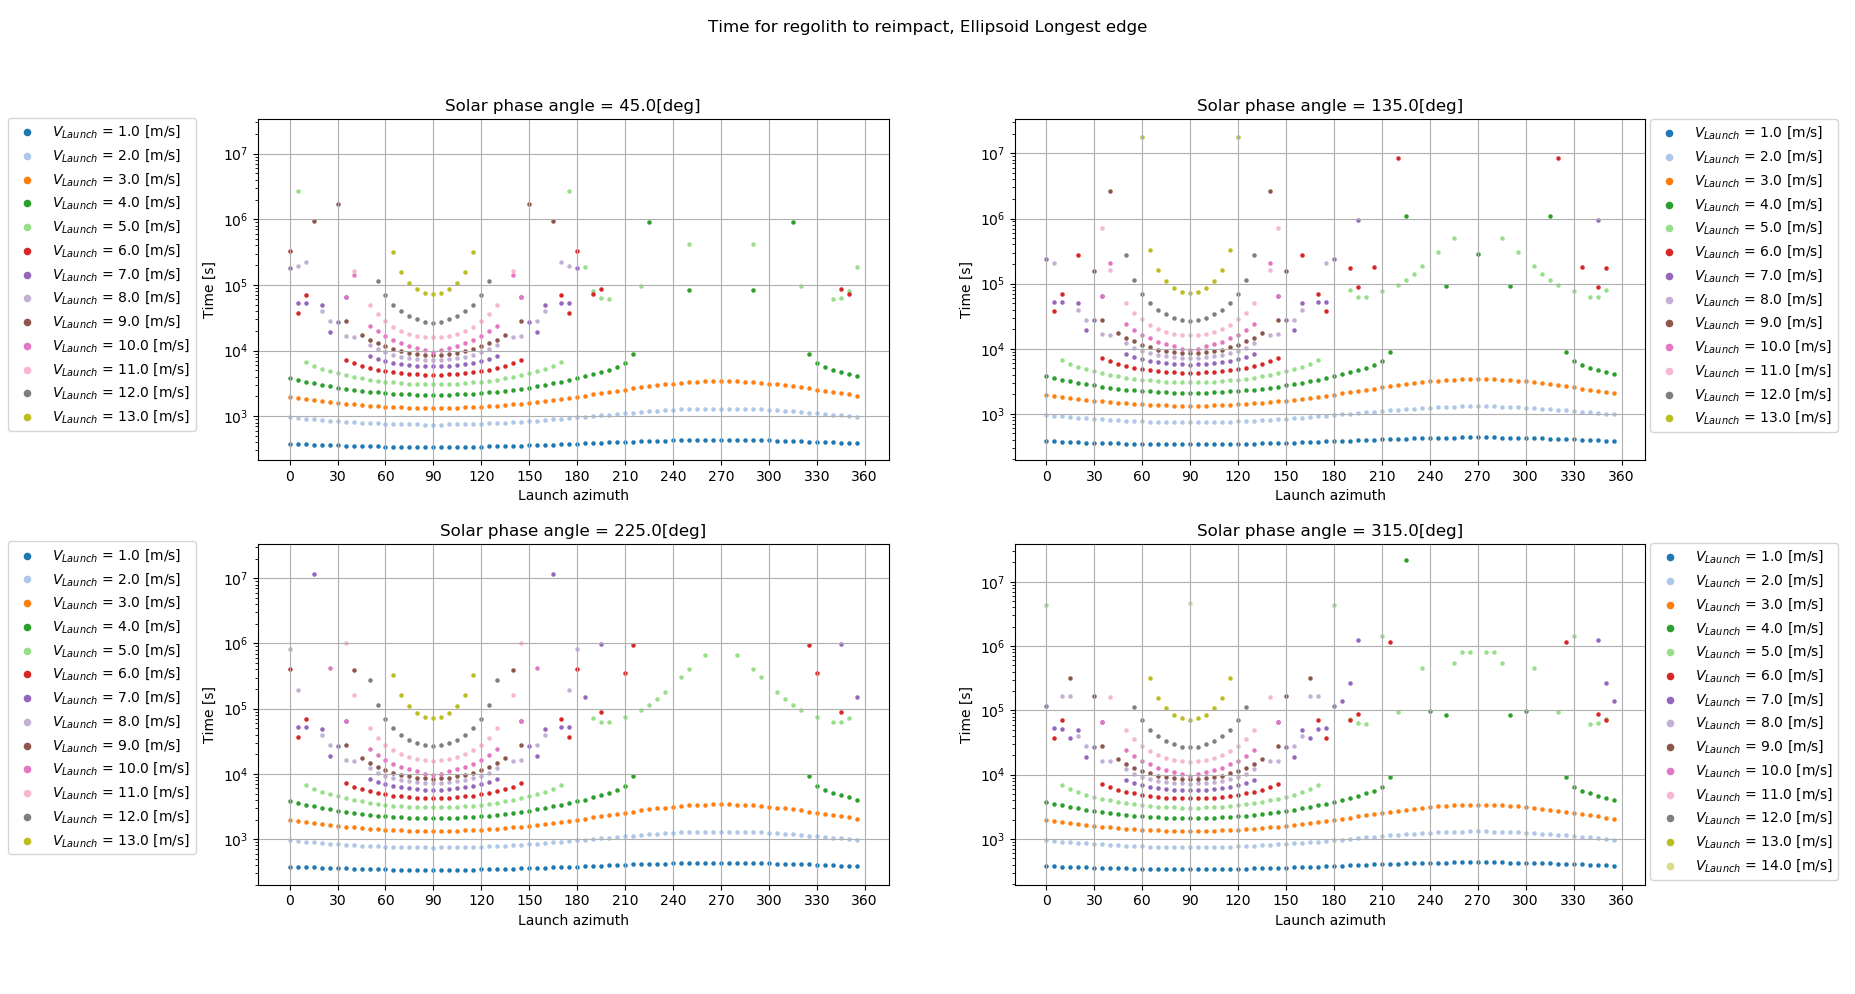
\includegraphics[angle=90, width=\textwidth, height=\textheight]{longest_edge_perturbations/3.2Density_1cmSize/time_to_reimpact_all_solar_phases.png}
\caption{Time taken by regolith at different velocities and launch directions to re-impact with the surface of the asteroid. Particle code LoGSP-1.}
\label{fig:LoGSP_1_reimpact_time}
\end{figure}
\FloatBarrier
%%%
We shall now look at the cases where the lofted regolith gets (temporarily) captured in orbit by the asteroid. The initial conditions for all capture cases, for the current particle size and density, were mentioned earlier in \Cref{tab:LoGSP_1_capture}.
